\documentclass[12pt,a4paper]{article}
\usepackage[utf8]{inputenc}
\usepackage[T1]{fontenc}
\usepackage[polish]{babel}
\usepackage{amsmath}
\usepackage{amsfonts}
\usepackage{amssymb}
\usepackage{graphicx}
\usepackage{hyperref}
\usepackage{xcolor}
\usepackage{float}
\usepackage{geometry}
\geometry{a4paper, margin=2.5cm}

\title{Technologia od podstaw}
\author{Marcin Pawlak}
\date{\today}

\begin{document}

\maketitle

\section{Wstęp do praktycznej realizacji projektu}

Niniejszy raport ma charakter wybitnie inżynierski i praktyczny. Stanowi on swego rodzaju dziennik deweloperski (tzw. \textit{Proof of Concept}), w którym krok po kroku opisuję fizyczną realizację systemu nadzorowania obiektów. Zamierzam tu pokazać czystą mechanikę -- od zakupu i konfiguracji pierwszego testowego czujnika ruchu za przysłowiowe grosze, aż po wyświetlenie wielkiego informacyjnego komunikatu o statusie pojedynczej sali na ekranie telewizora powieszonego w holu wydziału studenckiego.

Przełożenie zarysowanej wcześniej teorii na urządzenia z układami scalonymi wymaga absolutnego porządku, który realizowany będzie według ściśle ustalonego planu wdrożeniowego:

\begin{enumerate}
    \item \textbf{Kupno taniego czujnika Zigbee (PIR) na testy:} Na sam start projektu zamawiamy najprostszy z możliwych, najtańszy czujnik ruchu (za ok. 20-30 zł). Ma on spełnić jedno proste zadanie rzucone mi na biurko -- zyskać dowód na to, że potrafimy go w ogóle poprawnie sparować i jesteśmy w stanie odczytać prosty sygnał o wzroście napięcia (ruch wyłapany przez soczewkę) prosto na ekranie domowego komputera.
    
    \item \textbf{Konfiguracja lokalnej bramki (Dongle USB):} Kolejnym etapem opisanym poniżej będzie fizyczne podpięcie tak zwanego "gwizdka" w roli odbiornika USB bezpośrednio do portu stacji bazowej. Chcemy uniknąć podpinania czujników pod serwery amerykańskie czy azjatyckie w chmurze – stąd nacisk na stworzenie własnej, bardzo prywatnej sieci Zigbee pracującej wyłącznie w przestrzeni lokalnej po kablach i routerze wewnętrznym uczelni.
    
    \item \textbf{Testy "w boju" i zmiana na twarde czujniki milimetrowe (mmWave):} Rozumiejąc na tanich testerach, z czym je się odbieranie surowych sygnałów cyfrowych, pozbędziemy się przestarzałych zabawek PIR. W ich miejsce zamontujemy docelowe procesory o potężnej czułości (radary mmWave). Ich przewaga zadba o brak tzw. "ślepych łatek" -- radary te wychwycą studenta w auli nawet w momencie, gdy siedzi on przez godzinę praktycznie całkowicie bez ruchu, odrabiając projekty i nie dając standardowym czujnikom termicznym dowodów na swoje istnienie w danej strefie.
    
    \item \textbf{Przesłanie wiadomości (Pingów) do docelowego systemu:} Zaprogramowanie systemu backendowego. Logika serwera będzie napisana i skonfigurowana tak, by rutynowo -- w cyklu np. równo co 60 sekund -- logowała się i pobierała zaktualizowany stan czujników sprzętowych. Po zebraniu odczytów, mikrokontroler wypluje z siebie bardzo krótką, ważącą zaledwie kilkanaście kilobajtów formatkę (plik JSON) z oceną zajętości w głąb potężnej sieci lokalnej pozwalając na jej wyświetlenie.
    
    \item \textbf{Stworzenie ekranu w lobby (Końcówka Front-endowa):} Wisienka na inżynierskim torcie. Wyciągnę gotowy i oszlifowany ułamek danych z serwera, ładując go tym razem w postaci wielkiego i czytelnego piktogramu do telewizora wejściowego. Wyświetlimy po prostu wielki, kolorowy napis: \textcolor{green}{\textbf{„Sala 401: WOLNA”}} lub \textcolor{red}{\textbf{„Sala 401: ZAJĘTA”}}. Dowiedzie to faktu, że przeskok wymiarowy od płytki lutowanej po warstwę socjalną jest niezwykle prosto funkcjonującym mechanizmem obwodu zamkniętego.
\end{enumerate}

Tak skrojona struktura raportu sprawnie obroni przed audytami i promotorami udaną koncepcję wdrożenia naszego rozwiązania inżynieryjnego z etapu koncepcyjnego do fazy namacalnej.

\section{Kupno i montaż pierwszego sprzętu testowego}

\subsection{Wybór budżetowego czujnika ruchu (PIR)}

Decydując się na tak zaawansowany projekt architektoniczny obwodu zamkniętego, wprowadziliśmy strategię optymalizacji ryzyka kosztowego do projektu. Zamiast inwestować potężny uczelniany budżet w profesjonalny, bardzo drogi sprzęt radarowy \textit{mmWave} z firmy instalatorskiej, gdzie na tym etapie nie mieliśmy nawet żadnej pewności zestawienia anten – do podstawowych testów programistycznych sprowadzono bardzo tani sprzęt komercyjny. 

Zakupiony \textit{Proof of Concept} to klasyczny czujnik bazujący mechanicznie na taniej soczewce \textbf{PIR} (\textit{Passive Infrared}). Technologia ta ma zerową inteligencję i odnotowuje po prostu skokowe wahania plam ciepła w strefie. Dokładną nazwę i model naszego zakupionego urządzenia widać poniżej. W specyfikacji układu nadawczego czujnik ten zasilany jest zwykłą wymienną baterią typu pastylka, obiecując rzucenie w eter wygenerowanego protokołu operacyjnego Zigbee. 

\begin{figure}[H]
    \centering
    % Zrzut ekranu wycentrowany na szerokość strony
    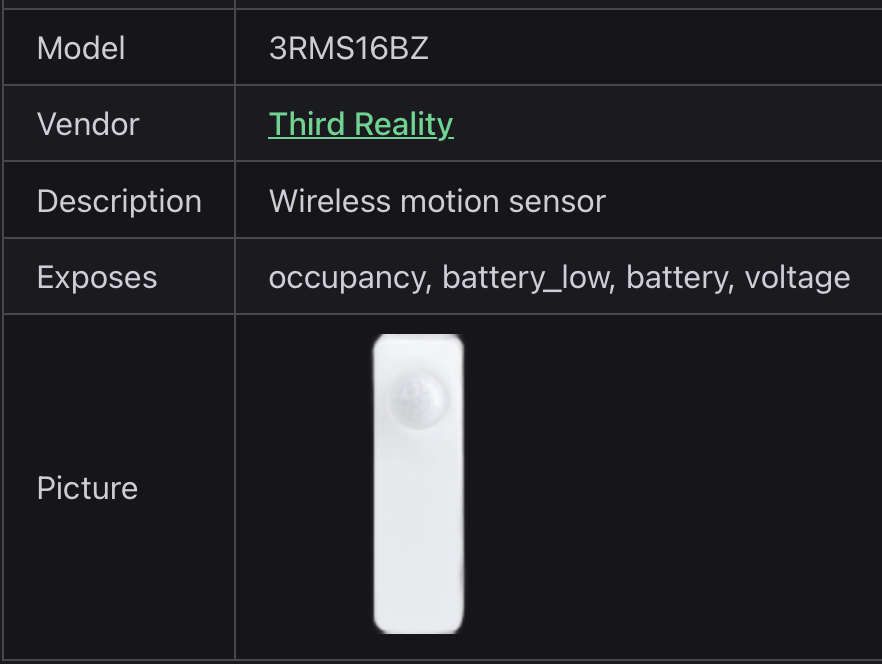
\includegraphics[width=0.9\textwidth]{zrzut.png}
    \vspace{0.6cm} % Mały odstęp pionowy
    
    % Dwa fizyczne zdjęcia ułożone pięknie obok siebie w jednej poziomej linii
    \begin{minipage}{0.48\textwidth}
        \centering
        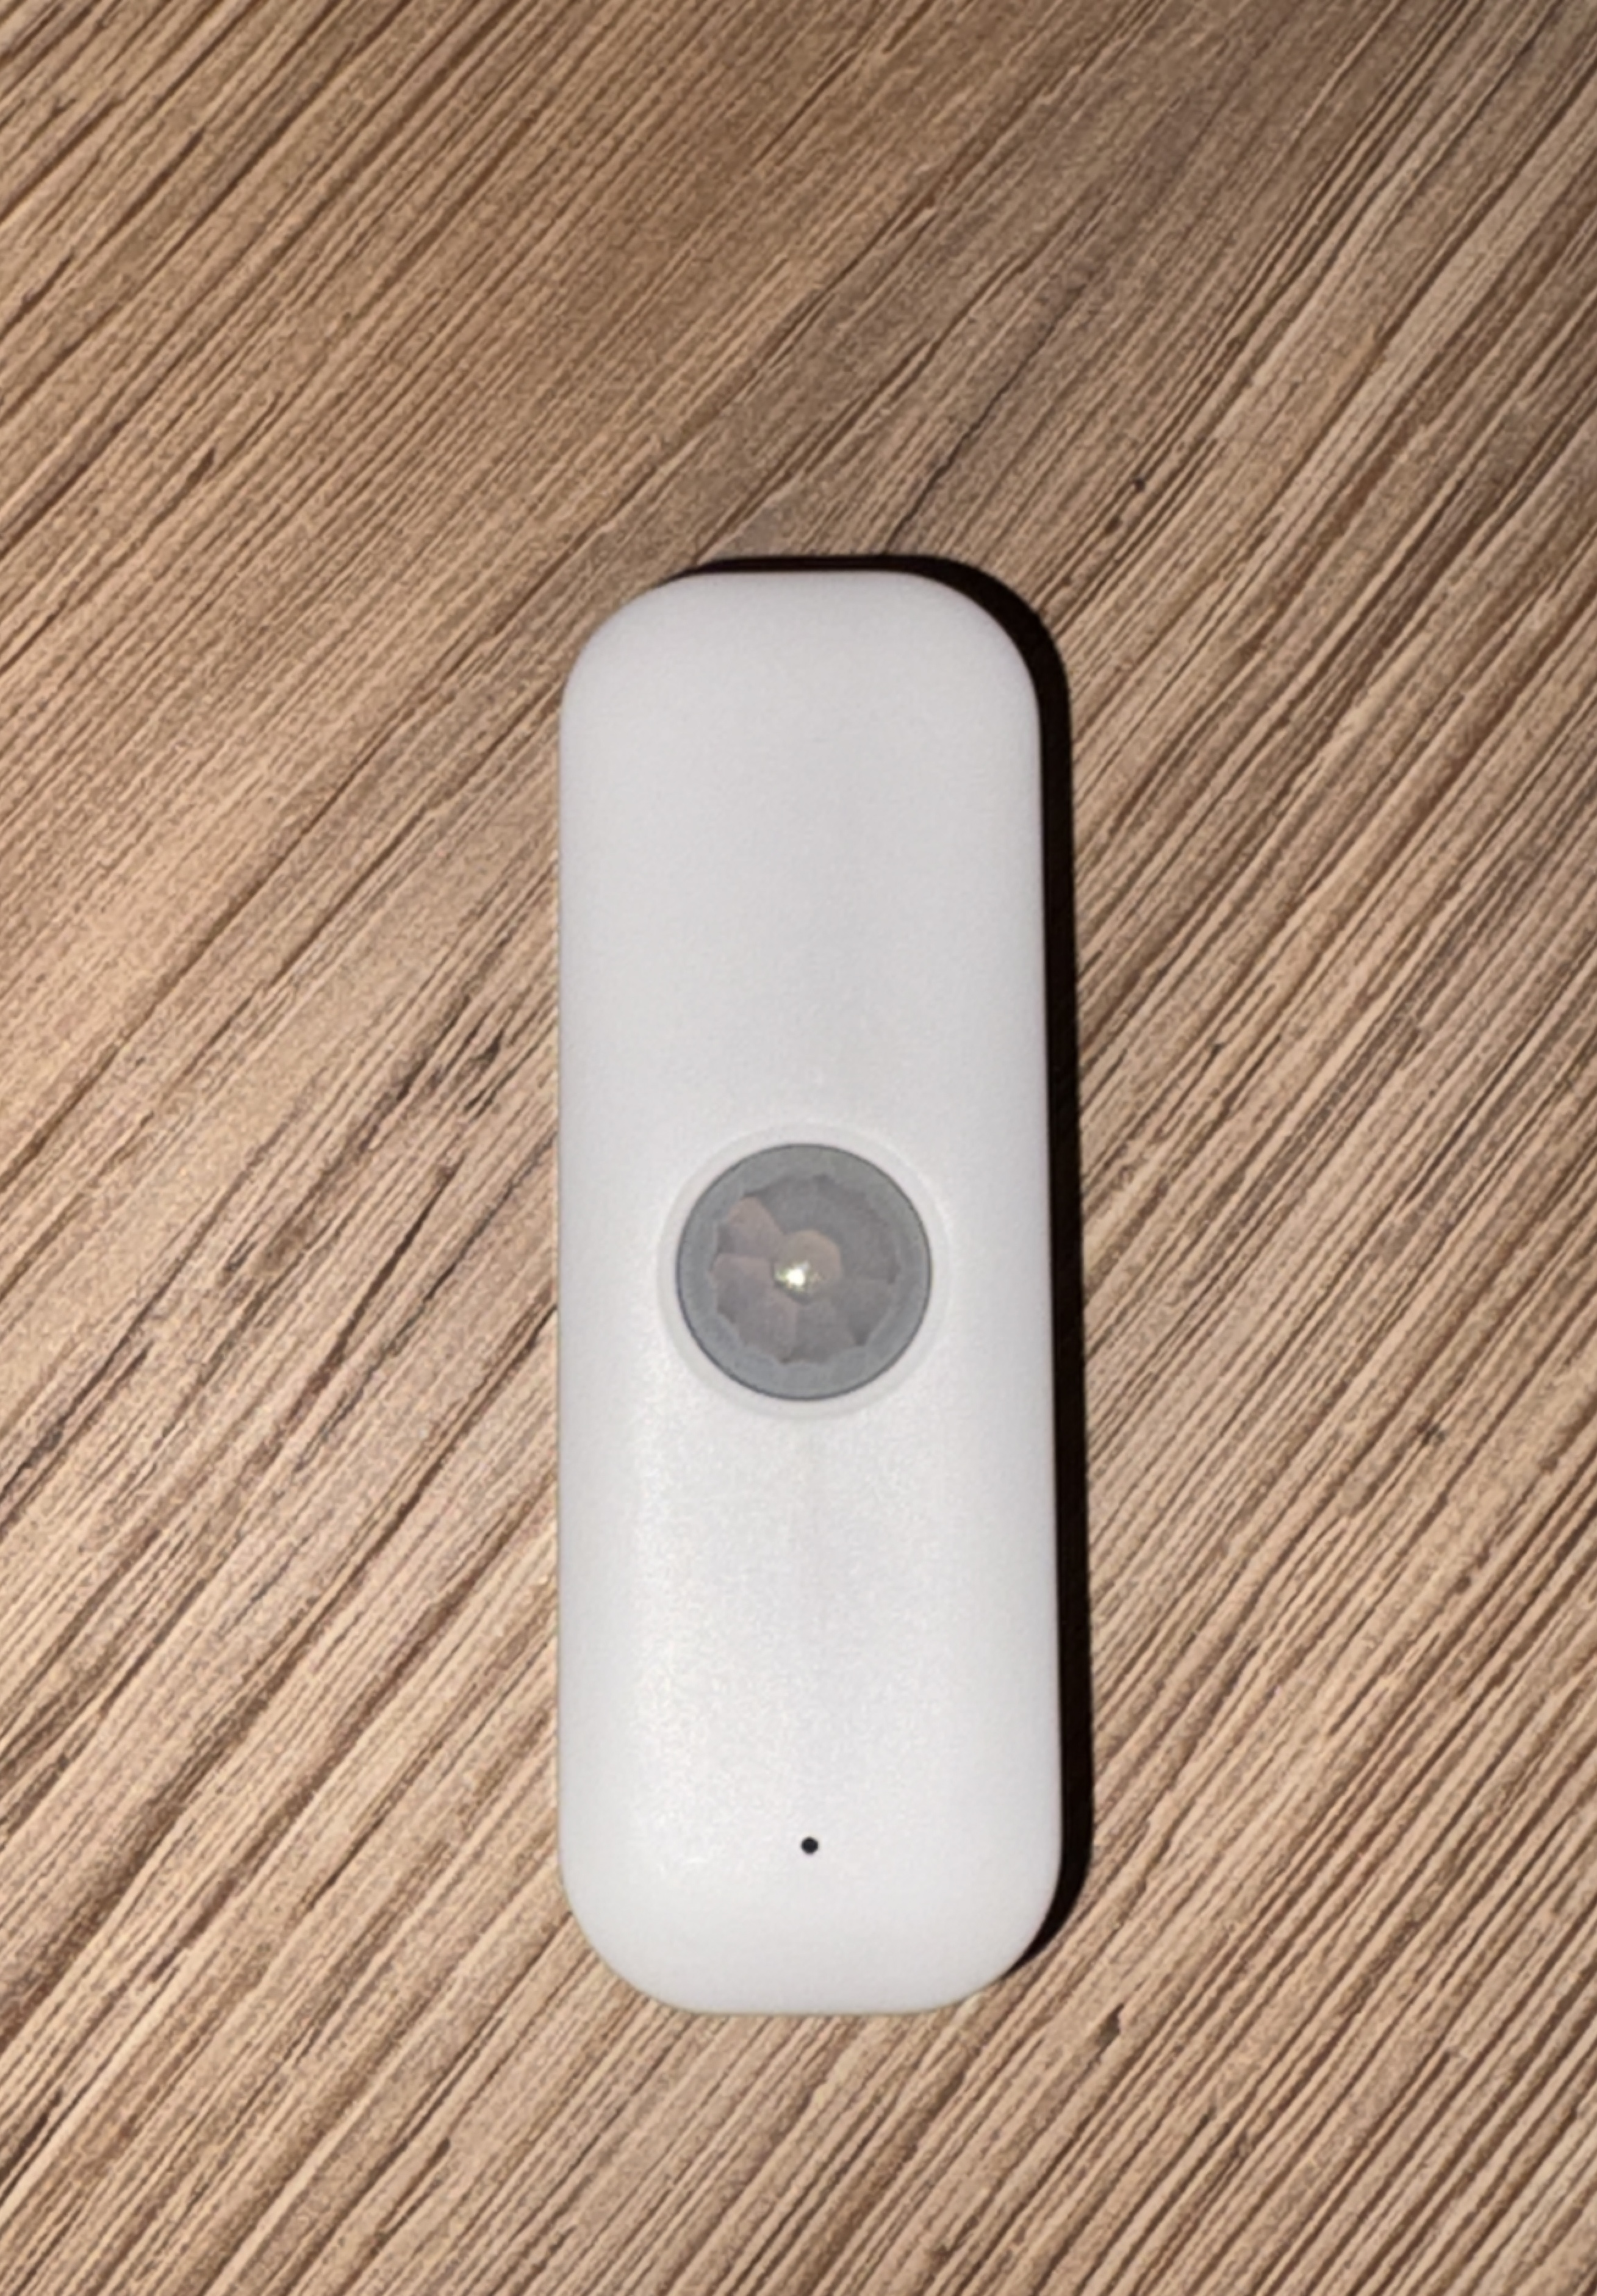
\includegraphics[width=\linewidth]{IMG_4774.JPG}
    \end{minipage}\hfill
    \begin{minipage}{0.48\textwidth}
        \centering
        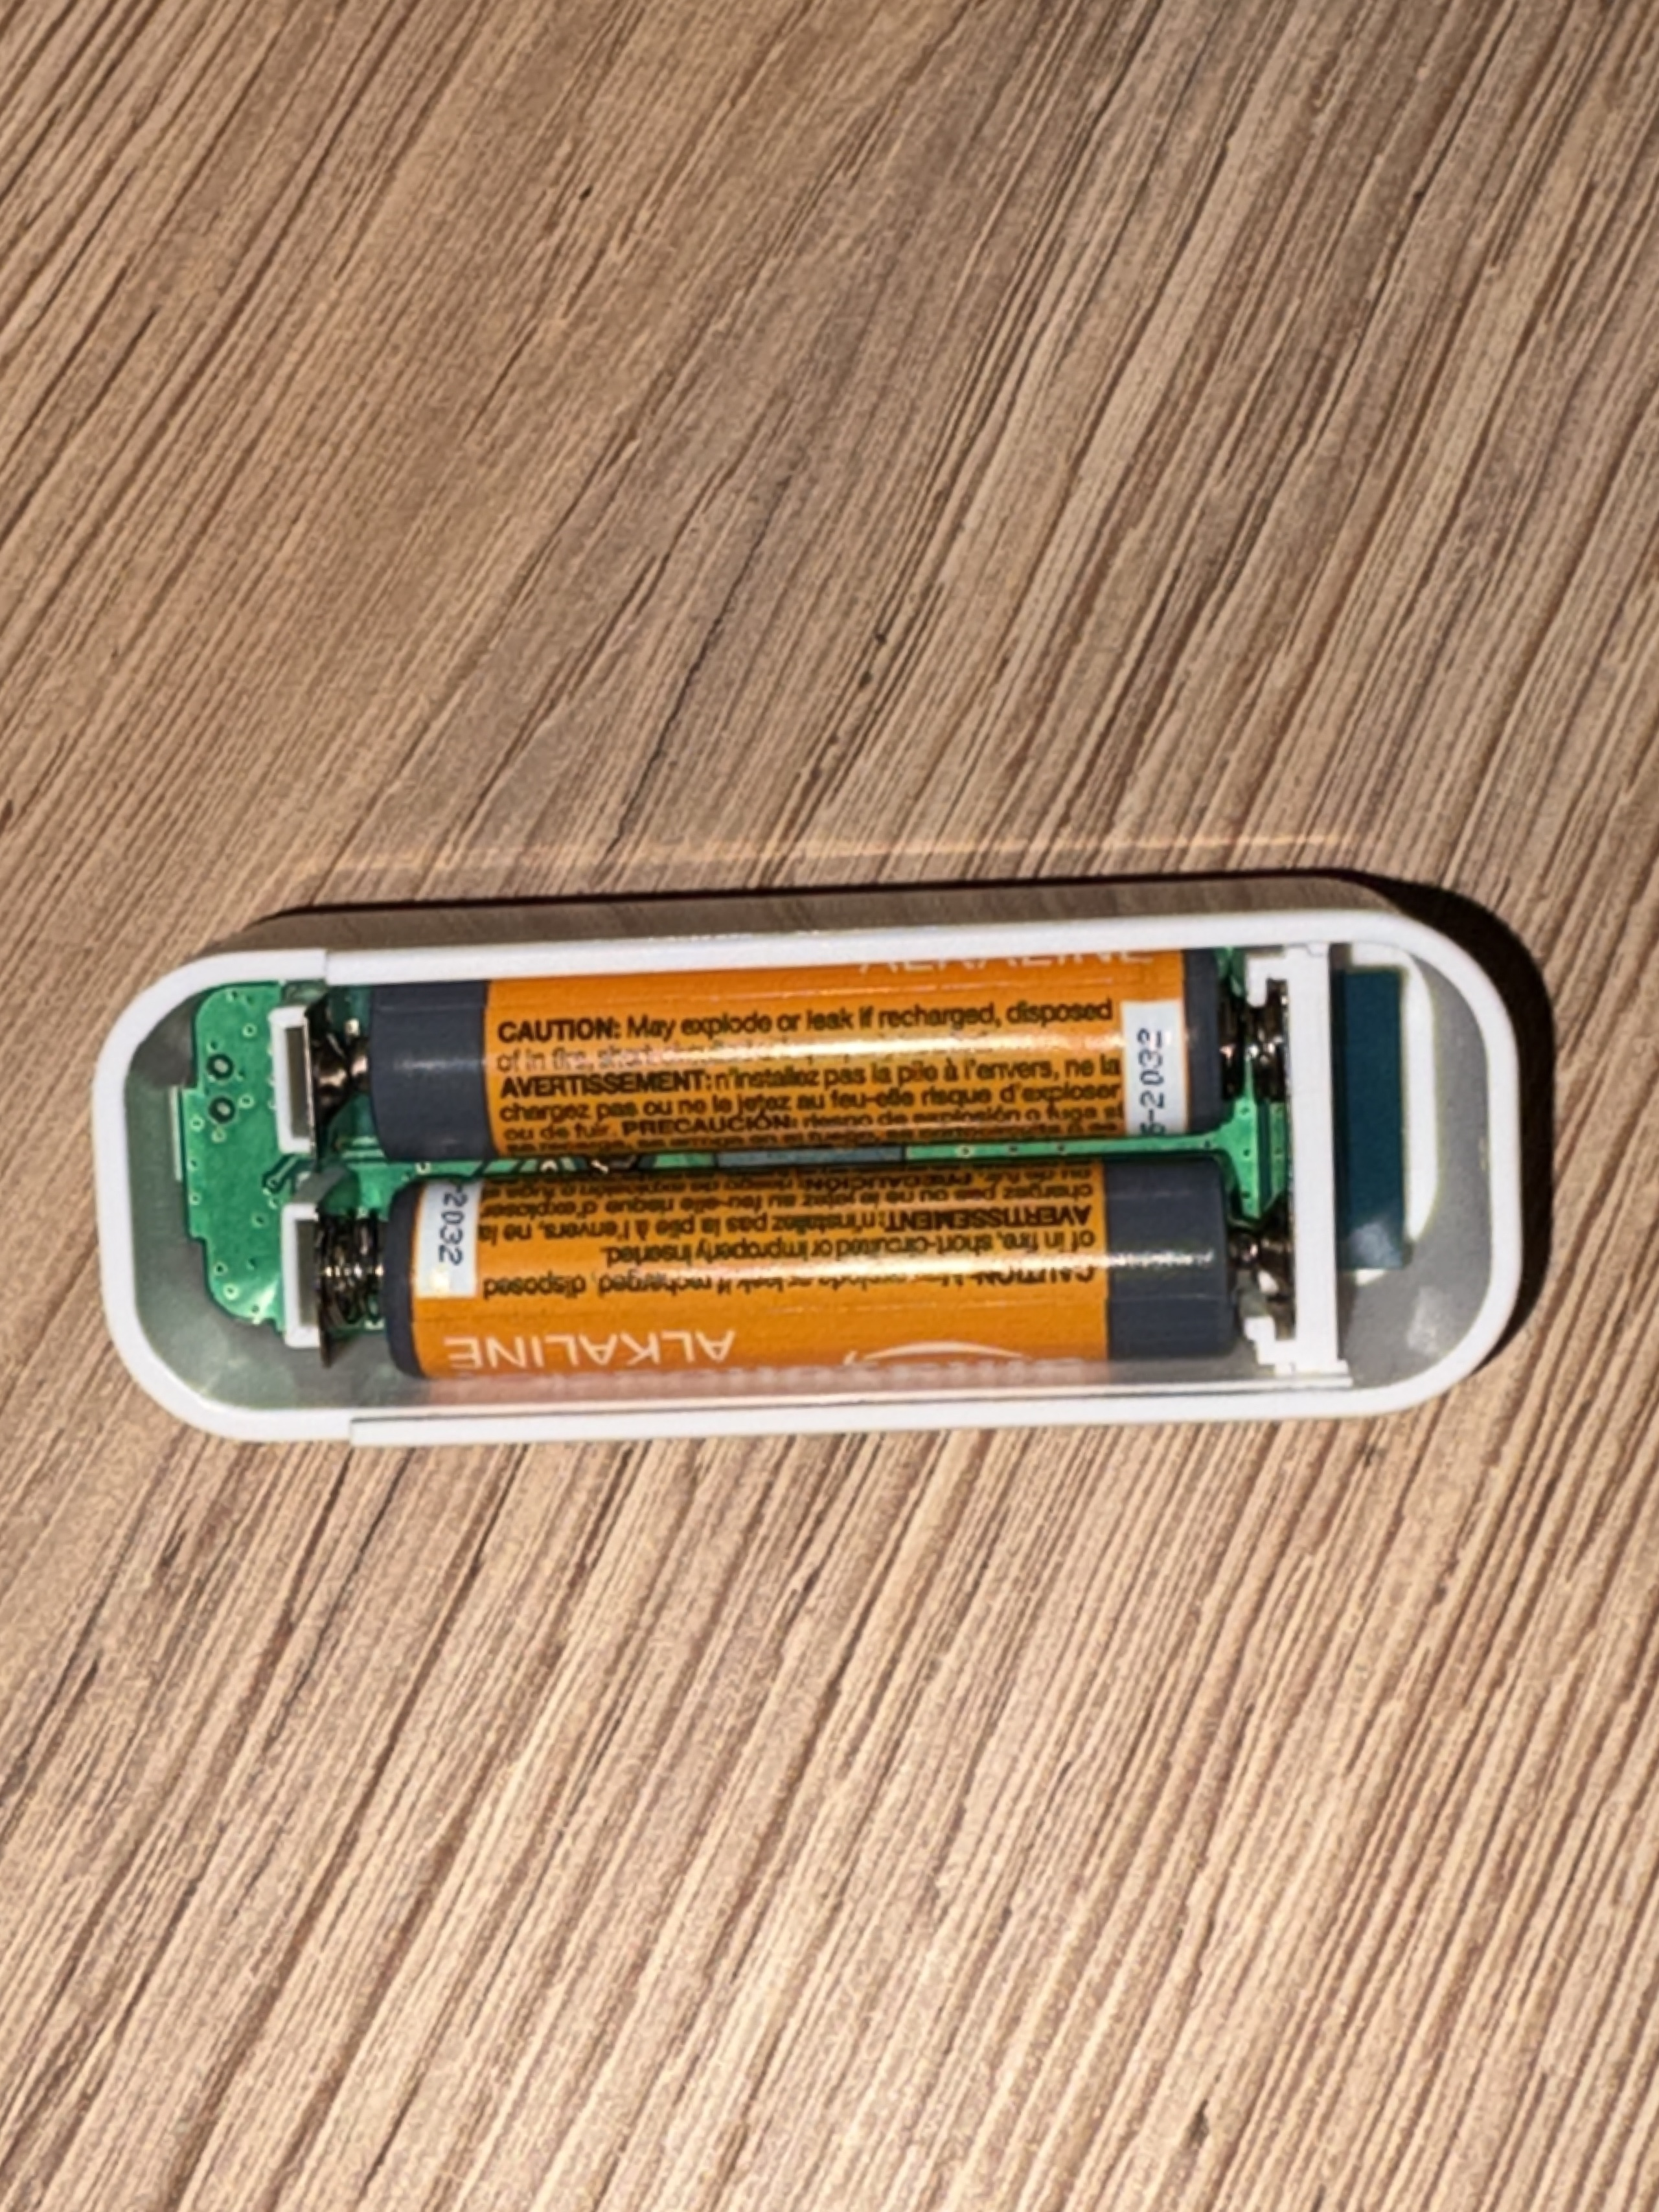
\includegraphics[width=\linewidth]{IMG_4775.JPG}
    \end{minipage}
    
    \caption{Skonfigurowany testowy czujnik PIR: parametry pracy odczytywane w systemie (góra) oraz jego bardzo prosta budowa obudowy (na dole).}
    \label{fig:zakupiony_czujnik}
\end{figure}

\section{Łączenie czujnika z komputerem}

Kolejnym kluczowym krokiem po fizycznym zakupie i aktywacji sprzętu była integracja urządzenia z naszą jednostką sterującą. Do nawiązania komunikacji wykorzystano chmurę producenta oraz platformę dla deweloperów -- Tuya IoT.

Warto podkreślić, że strona Tuya dostarcza nie tylko prosty, graficzny panel zarządzania, ale udostępnia pełnoprawne i zaawansowane środowisko programistyczne. Z poziomu panelu deweloperskiego można wygenerować specjalne klucze uwierzytelniające, które pozwalają na bezpieczne łączenie rozwiązań Tuya z naszym własnym, lokalnym komputerem za pośrednictwem rozbudowanego interfejsu API. 

Wydzielona dedykowana struktura API oznacza ogromną elastyczność -- komputer może przejąć na siebie ciężar wysyłania komend czy odbierania statusów wysyłając zapytania wprost w mechanizmy platformy Tuya, która następnie przepchnie żądanie do żarówki lub przyśle nam informację z czujnika. Tego typu rozwiązanie jest standardem w rozwiązaniach informatycznych w architekturze mikrousług.

\end{document}
